%%
%% This is file `sample-sigconf.tex',
%% generated with the docstrip utility.
%%
%% The original source files were:
%%
%% samples.dtx  (with options: `sigconf')
%% 
%% IMPORTANT NOTICE:
%% 
%% For the copyright see the source file.
%% 
%% Any modified versions of this file must be renamed
%% with new filenames distinct from sample-sigconf.tex.
%% 
%% For distribution of the original source see the terms
%% for copying and modification in the file samples.dtx.
%% 
%% This generated file may be distributed as long as the
%% original source files, as listed above, are part of the
%% same distribution. (The sources need not necessarily be
%% in the same archive or directory.)
%%
%% The first command in your LaTeX source must be the \documentclass command.
\documentclass[sigconf]{acmart}
\settopmatter{printacmref=false} % Removes citation information below abstract
\renewcommand\footnotetextcopyrightpermission[1]{} % removes footnote with conference information in first column


%%
%% \BibTeX command to typeset BibTeX logo in the docs
\AtBeginDocument{%
  \providecommand\BibTeX{{%
    \normalfont B\kern-0.5em{\scshape i\kern-0.25em b}\kern-0.8em\TeX}}}

%% Rights management information.  This information is sent to you
%% when you complete the rights form.  These commands have SAMPLE
%% values in them; it is your responsibility as an author to replace
%% the commands and values with those provided to you when you
%% complete the rights form.
\setcopyright{none}
%copyrightyear{2018}
%\acmYear{2018}
%\acmDOI{10.1145/1122445.1122456}

%% These commands are for a PROCEEDINGS abstract or paper.
%\acmConference[Woodstock '18]{Woodstock '18: ACM Symposium on Neural
%  Gaze Detection}{June 03--05, 2018}{Woodstock, NY}
%\acmBooktitle{Woodstock '18: ACM Symposium on Neural Gaze Detection,
%  June 03--05, 2018, Woodstock, NY}
%\acmPrice{15.00}
%\acmISBN{978-1-4503-XXXX-X/18/06}


%%
%% Submission ID.
%% Use this when submitting an article to a sponsored event. You'll
%% receive a unique submission ID from the organizers
%% of the event, and this ID should be used as the parameter to this command.
%%\acmSubmissionID{123-A56-BU3}

%%
%% The majority of ACM publications use numbered citations and
%% references.  The command \citestyle{authoryear} switches to the
%% "author year" style.
%%
%% If you are preparing content for an event
%% sponsored by ACM SIGGRAPH, you must use the "author year" style of
%% citations and references.
%% Uncommenting
%% the next command will enable that style.
%%\citestyle{acmauthoryear}

%%
%% end of the preamble, start of the body of the document source.
\begin{document}

%%
%% The "title" command has an optional parameter,
%% allowing the author to define a "short title" to be used in page headers.
\title{Working Title: Quantitative Privacy Analysis of using Kadcast for Transaction Broadcasting}

%%
%% The "author" command and its associated commands are used to define
%% the authors and their affiliations.
%% Of note is the shared affiliation of the first two authors, and the
%% "authornote" and "authornotemark" commands
%% used to denote shared contribution to the research.

\author{John Smith}
\affiliation{\institution{The Th{\o}rv{\"a}ld Group}}
\email{jsmith@affiliation.org}

\author{Julius P. Kumquat}
\affiliation{\institution{The Kumquat Consortium}}
\email{jpkumquat@consortium.net}

%%
%% By default, the full list of authors will be used in the page
%% headers. Often, this list is too long, and will overlap
%% other information printed in the page headers. This command allows
%% the author to define a more concise list
%% of authors' names for this purpose.
\renewcommand{\shortauthors}{Trovato and Tobin, et al.}

%%
%% The abstract is a short summary of the work to be presented in the
%% article.
\begin{abstract}
\section{Abstract}
When discussing the privacy of blockchains or Distributed Ledger Technologies, the
focus of the analysis is often on the consensus layer of the blockchain.
Another major factor for a comprehensive privacy analysis is
the network layer, which defines how messages are passed between peers.
On this layer many privacy sensitive informations like public IP addresses of users and connections between the peers
of the network are used and can potentially be recorded by malicious parties.
In this report we will do a simulation based, quantitative privacy analysis of the Kademlia inspired
network overlay Kadcast, that can be used for efficient broadcasting e.g. in Bitcoin or other blockchain based technologies.
The focus of the anaylsis is the usage of Kadcast for broadcasting transactions and the evaluation of an adversary's capability
of linking observed transactions to IP addresses.
  %A clear and well-documented \LaTeX\ document is presented as an
  %article formatted for publication by ACM in a conference proceedings
  %or journal publication. Based on the ``acmart'' document class, this
  %article presents and explains many of the common variations, as well
  %as many of the formatting elements an author may use in the
  %preparation of the documentation of their work.
\end{abstract}

%%
%% The code below is generated by the tool at http://dl.acm.org/ccs.cfm.
%% Please copy and paste the code instead of the example below.
%%
%\begin{CCSXML}
%<ccs2012>
% <concept>
%  <concept_id>10010520.10010553.10010562</concept_id>
%  <concept_desc>Computer systems organization~Embedded systems</concept_desc>
%  <concept_significance>500</concept_significance>
% </concept>
% <concept>
%  <concept_id>10010520.10010575.10010755</concept_id>
%  <concept_desc>Computer systems organization~Redundancy</concept_desc>
%  <concept_significance>300</concept_significance>
% </concept>
% <concept>
%  <concept_id>10010520.10010553.10010554</concept_id>
%  <concept_desc>Computer systems organization~Robotics</concept_desc>
% <concept_significance>100</concept_significance>
% </concept>
% <concept>
% <concept_id>10003033.10003083.10003095</concept_id>
%  <concept_desc>Networks~Network reliability</concept_desc>
%  <concept_significance>100</concept_significance>
%</concept>
%</ccs2012>
%\end{CCSXML}

%\ccsdesc[500]{Computer systems organization~Embedded systems}
%\ccsdesc[300]{Computer systems organization~Redundancy}
%\ccsdesc{Computer systems organization~Robotics}
%ccsdesc[100]{Networks~Network reliability}

%%
%% Keywords. The author(s) should pick words that accurately describe
%% the work being presented. Separate the keywords with commas.
%\keywords{datasets, neural networks, gaze detection, text tagging}



%%
%% This command processes the author and affiliation and title
%% information and builds the first part of the formatted document.
\maketitle
%\pagestyle{plain} % removes running headers

\section{Introduction}
So called ``Cryptocurrencies'' and other blockchain based technologies are gaining
increasing attention since the emergence of Bitcoin, both in the academic community and in media []. \\
%.[hier bessere ueberleitung]
These cryptocurrencies, like Bitcoin can be used analogous to fiat money to transfer ``coins''
from a sender to a receiver. In Bitcoin, new coins can be ``mined'' by investing computing power.
Unlike a fiat money transaction, which is generally handled by a bank, there is no central instance
that authorizes Bitcoin transactions. Instead Bitcoin is a peer-to-peer based system that is run publicly on the internet
and allows all participants to achieve consensus on a single valid transaction history without the need for a trusted third party.
Users can participate in the network via pseudonymous identities and there is no inherent link between a pseudonymous public identifier and a natural person,
albeit deanonymization attacks can be performed to potentially link the public key of a user to an IP address or even a real name [].
To store the transaction history, Bitcoin uses an append-only, distributed ledger (the so called ``blockchain'')
and consensus on the state of the ledger is periodically reached
by the participants of the network via a distributed consensus algorithm. [for detailed explanation refer to nakamoto paper]
Since payments and money flow comprise of very privacy sensitive information, and everyone can join the Bitcoin peer-to-peer network
and access the transaction history, the privacy of Blockchains has been an active research area since ...[].
There is a large amount of scientific literature [specifically] on the privacy of the consensus layer of
blockchains [], describing weaknesses [e.g using heuristics to construct entity graph, ...] and algorithms to mitigate privacy issues [mixing, coinjoin, zk-snarks, ...] [bib]. \\
Yet another important factor for a comprehensive privacy analysis is the network layer, which
defines how messages are passed between participants of the network.
Because of the open nature of public blockchains, any adversery can join the network and potentially gain access to
privacy sensitive information on the networking layer, like the IP addresses of peers they are connected to.
The gathered information can then be used to perform deanonymization attacks, e.g. to link transactions to public IP addresses [first described in Koshy]. \\
One of the most important jobs of the network layer in blockchains is to handle broadcast messages, since
both new blocks and new transactions are sent as broadcasts through the network.
While Bitcoin started with a relatively naive approach of broadcasting
new blocks and transactions in the network, by just iteratively spreading the
messages to all nearby nodes,
the network overlay of blockchains has since been revisited multiple times to optimize the message passing with regards to efficiency and privacy [Koshy, Bojja, Fanti, Rohrer, ...] and is continued to be researched and optimized []. \\
One [semi-]recently devoloped peer-to-peer overlay that can be used for efficient broadcasting in P2P networks is Kadcast.
Kadcast is a Kademlia based network overlay that diverges from the naive and redundant approach of ``gossiping'', to a structured message propagation, leveraging the bucket logic introduced by Kademlia, and achieving a complete network coverage with minimal messages (excluding neccessary redundancy for stability reasons). [TODO vllt infografik einfügen wie kadcast/bucket logic funktioniert?]
The initial application for Kadcast was to broadcast newly mined blocks.
Because the direct link between IP addresses and transactions is already
broken when a transaction is included in a block, the block propagation
was optimized for efficiency only, without any concerns for privacy issues. \\
However, when using Kadcast to broadcast transactions instead, an adversary that is connected to the network can potentially perform
deanonymization attacks and link transactions to the public IP addresses that issued them. \\
Since the travel path of messages in Kadcast is structured, and message redundancy is reduced to a minimum, the question was raised, what sorts of privacy implications using Kadcast as a broadcasting algorithm for transactions would have [R.]. \\
To start answering this question, we want to use a quantitative approach and perform a deanonymization attack
as it could happen in a real world scenario. Because of the lack of historical data, we use a [highly] abstracted network
simulation to generate data which then can be used for the attack. The simulation setup, including constraints of our simulation and potential resulting implications for the attack are described in [Section Simulation Setup]. \\
We further model our adversary and describe the means of our attacker, explaining
which simplifications we made to the attacker model, and why we can use such a simplified model
without sacrificing much effectiveness of the attack [Ch. atk.model]. \\
We will then shortly elaborate which metrics we applied to evaluate the impact of the attack [Ch. metrics]. \\
In our evalution we will take a closer look at the results of our simulated attacks, and
review if the privacy impacts of using Kadcast for transaction broadcasting align with our
research hypothesis, that the structured overlay has [negative] effects on the privacy of the network. \\
In the last step of our evalution, we will try to mitigate the privacy issues we have observed previously
by [prefixing /besseres wort] the broadcasts with an anonymity phase as described in [Dandelion]. \\
We conclude our analysis by briefly summarizing our results and giving an outlook
on where future research on this topic could be headed from this point on. \\
TODO Results + Outline



%\section{Evaluation}


\section{Simulation Setup}
For our simulation we used the discrete event simulation framework ``simpy''. \\
In our setup we do not incorporate network failures or change of any kind,
especially we do not have any dropped and corrupted messages or failing nodes. \\
%dropped and corrupted messages, network change, or byzantine nodes. \\
We run the simulation in two steps, starting with a setup phase, which
lets the nodes discover the network and fill their respective buckets and
after the network is stabilized we run the broadcast simulation phase. \\
Because we do not have any dropped messages, we set the redundancy parameter ``beta''
to 1, as it will always suffice to saturate the network. \\
We use latencies drawn at random from the iplane latency dataset[ref iplane] for all connections.




%- we start with setup phase and wait for all bootstrapping processes to finish and the network to stabilize
%- only then we start broadcasting

%- discrete event simulation, simpy
%- no dropped messages/churn -> beta set to 1
%- no fec

\section{Attacker Model\label{attacker_model}}
The overall goal of the attacker in our setup is to deanonymize users in
the network.
More precisely, the attacker wants to map transactions to the public IP addresses that issued them. \\
The Kadcast protocol comes with inherit security properties that mitigate different kind of attacks
and allow us to concisely define the means of an attacker if we assume
those properties hold []. [TODO: short summary of threat model of
kadcast, see kadcast paper] \\
The factor that is most important for mitigating attacks on the network layer, is that participants are
not allowed to choose their position in the overlay freely, and it is instead bound to the public IP address of a peer [].
The IP to ID mapping is done via a cryptographic hash function we assume to be unbreakable.
This makes it considerably harder for attackers to e.g. perform eclipse attacks [] or benefit in other ways from
a freely chosen position in the network. [sybil.] \\
We currently only know of two ways a malicious party that disobeys the
protocol could attack or observe the network differently than an ``honest-but-curious" attacker. \\
Those are namely a denial-of-service attack and an attack in which the adversary tries to flood
benign nodes with ping messages in hope of hitting the time frame in which the benign node has at least one unresponsive
peer, but has yet to refresh its peer list [eclipsing false friends]. In
this case the attacker could potentially insert their own nodes into the
peer list of the benign node.
This attack is made harder in Kadcast because not only does a node need
to have any arbitrary unresponsive peer, but an unresponsive peer
in the same bucket which the adversial node would be placed in. \\
Because of the assumed limited advantages byzantine nodes give an attacker and because our simulation setup doesn't account for any network change and turn,
which would be needed to perform a pinging attack as described above,
we exclude both of these attack vectors from our evalution and instead focus solely on an ``honest-but-curious" attacker. \\
For our analysis we further assume the adversary does not take the
network topology or their overlay-protocol knowledge into account
and only uses information recorded by the spies, including aggregated
and infered information. \\
This also means we assume the adversary does not utilize the broadcasting height attached to each broadcast message
for the deanonymization attack. While we do not formally show the impact
of not using that information,
this assumption can at least be somewhat justified by assuming the broadcasting height can
be hidden or masked to a certain extend (e.g. by sending the same message at different/randomized heights). \\
Under the specified circumstances we found the most realistic scenario
to be a botnet-like adversary that is part of the normal network overlay
and is used to deanonymize other users in the network. \\
We therefore model the attacker as an entity that controls a certain share of nodes in the network (so called ``spies'').
These spies all behave indistinguishably to benign nodes from an outsider's perspective (i.e. they obey the protocol). \\
To perform a deanynomization attack, the adversary logs all messages their nodes receive,
including timestamp and sender (IP address) for each recorded message. After the collection phase,
the attacker feeds the aggregated information up to this point in time into an estimator that
computes macro averaged precision and recall values over the whole dataset as defined in
Section~\ref{metrics}. \\
As an estimator we use the simple ``first-spy-estimator'' [ref].
This estimator maps every transaction to the first IP address that
sent the transaction to any of the spies. \\
Using this setup, it follows that anonymity is evaluated as a
network-wide property. Our evaluation does not incorporate the
perspective of a singular participating user of the network, i.e. we
make no claims on the anonymity of an individual participant of
the network, but only on the anonymity of the network as a whole.


\section{Anonymity Metrics}
The result of each of our deanonymization attacks is a transaction to IP mapping,
in which each observed transaction is mapped to exactly on IP address. \\
Our problem resembles a standard classification problem, as we try to assign each
transaction to a class (node). Therefore we can use standard classification metrics to
evaluate the effectiveness of our estimator.
We decided to compute averaged precision and recall values over the whole mapping,
as these are established and tested metrics for our use case [fanti et. al]. \\
The recall value can be interpreted as ``probality of detection'' and the
precision value relates inversely to the average plausible deniability per node.
That means, the higher the recall, the more likely it is that a random transaction
was correctly classified. The lower the precision, the greater the average plausible
deniability per node. \\
The values are computed as follows: [hier formel einfügen]


\section{Evaluation}
To evaluate the privacy properties of Kadcast we ran multiple simulations of
transaction broadcasting with the Kadcast algortihm. Each simulation has
the same amount of overall active nodes in the network and overall sent transactions.
We run each simulation for different percentages of spies. \\
The transactions are sent only by benign nodes, and all transactions are
randomly distributed among the sending nodes. Not each node does have to
send a transaction and some nodes may send multiple transactions. \\

First, we took a look at how the first spy estimator would perform in a standard setting,
using Kadcast with parameters used in ``real world scenarios'', i.e. a
bucket size of 20. \\

\begin{figure}
  \centering
      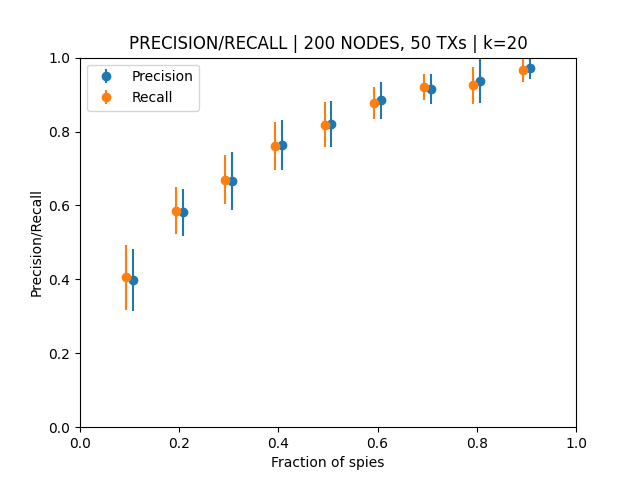
\includegraphics[width=0.5\textwidth]{figs/nodand}
  \caption{First Spy Estimator Kadcast}
  \label{fig:nodand}
\end{figure}

\begin{figure}
  \centering
      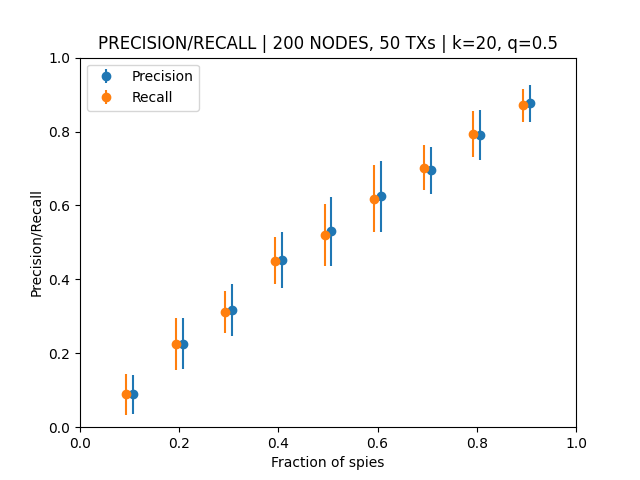
\includegraphics[width=0.5\textwidth]{figs/dand05}
  \caption{First Spy Estimator Kadcast with Dandelion}
  \label{fig:dand}
\end{figure}

The results can be seen in \ref{fig:nodand}. The figure include averaged
precision/recall values and the standard deviation of our measurements. \\
We see that the first spy estimator performs relatively well. \\
Even with an amount of as low as 20\% of spies, the attacker can
map over half of the sent transactions correctly. This is very far from
the best case scenario [TODO which is?]. \\

Just out of curiousity we wanted to test if the bucket size has any
meaningful correlation to the performance of the estimator. We therefore
repeated our experiment with common bucket sizes, the results can be
seen in [TABLE1].
Different k values did not have a positive effect on the anonymity
properties. \\

We further wanted to know if we can improve the anonymity by using dandelion spreading.
We therefore implemented a simple version of the dandelion algorithm. It
uses the ``q'' parameter as described in the original dandelion paper,
to decide at each hop if the algorithm should stop the anonymity phase
and start the broadcasting phase. The q value is the probability to leave
the anonymity phase at a hop. We did not build a Hamiltonian circuit as
described in the paper, but just used a random (loopfree) path through
the graph for each transaction. Therefore our approach is a simplified
version of dandelion, a little more akin to regular
``diffusion-by-proxy''. Nevertheless this approach has some observable
positive effects on the anonymity of our network. The result for
combining Kadcast with this simple implementation of dandelion, using
the standard parameter $q = 0.5$, can be seen in \ref{fig:dand}. Compared to
standard Kadcast spreading this is a massive improvement. \\
We ran the experiment again with different $q$ values, the results can
be seen in [TABLE2]. \\
As Dandelion only adds a constant overhead to spreading [source
dand1fanti], we think it would be a meaningful addition to Kadcast,
especially if we take the bad results we have observed in our standard
Kadcast experiments into consideration.


- auf bucket reihenfolge eingehen
- k ändern
- bucket reihenfolge ändern
- std deviation/x samples/...


\section{Discussion}
Our results indicate that the privacy properties of kadcast are not optimal. \\



[ DISCUSS RESULTS HERE ]



In our analysis we assumed the adversary does not take the network topology into account.
It would be interesting to drop this assumption and do further research on what kind of
information a less ``naive'' attacker could exploit. \\
For example, one could explore if it would be possible for an attacker to infer additional information
about the bucket layout of sending nodes, and use this information to create a more sophisticated estimator. \\
If the attacker could somehow identify some nodes as being far away or close by (according to the XOR distance),
they could e.g. weight their obvervations by proximity, as a close node has a higher chance to have a direct link
to a node. \\

To really understand the bounderies of an attack, it would further be of interest to
investigate the symmetry properties of the message spreading. \\
In general, it would be of great benefit if our results were reinforced either
by a more realistic simulation that closer resembles real world scenarios, e.g. including failures, or
by a formal modal that gives a better understanding of an attackers capabilites.


%We do not know yet, if there is no possibility an adversary could 

%Also, if an adversary can somehow identify ``proximity clusters'' of nodes, i.e. nodes that are
%grouped close together from an adversarys node perspective, this information could be used
%to weight observations by clusters, because such a cluster would deviate in the amount
%of direct links it has to the spy (a cluster of close nodes will have many direct links to the spy,
%whilst a cluster of far away nodes does have few direct links to the spy)

%such clusters(or proximity in general) could maybe be inferred by combining observations?
%-> even better: know if nodes are close, far
%[Ich hab mir zwar Überlegungen dazu gemacht, aber bin zu keinem Ergebnis gekommen.
%Die Grundidee war, dass wenn wir einen Weg finden Rückschlüsse auf das Bucket Layout des initialen Senders zu bekommen
%(z.B. mit einer Heuristik anhand der message timestamps?), dann könnte man evtl. erkennen welche der eigenen adversary
%Knoten aus Broadcast Initiator Sicht geringe Entfernung haben und damit evtl. irgendwas anfangen. Vllt. ausprobieren
%ob eine Gewichtung Sinn macht, da die Chance einen direkten Link zum Initiatior zu haben ja größer wird je näher man ihm kommt.
%Auch wenn man nur Teilinformationen bekommen kann, z.B. das bestimmte eigene Knoten aus Broadcaster Sicht ein ``Proximitätscluster''
%bilden, könnte man das evtl. für den Estimator benutzen, da ein solches Cluster ja entweder überdurchschnittlich viele
%oder überdurchschnittlich wenige direkte Verbindungen zum Broadcaster haben muss (je nachdem ob es nah oder fern liegt).
%Leider bin ich auf keine Möglichkeit gekommen solche Erkenntnise als Angreifer zu erlangen.
%]
%This also means we assume the adversary does not take the broadcasting height attached to each broadcast message into account
%for the deanonymization attack. While we do not formally show the impact of not using this information,
%this assumption can at least be somewhat justified because the broadcasting height can
%theoratically be hidden or masked to a certain extend (e.g. by sending the same message at different/randomized heights).


%- would be nice to have math. model/good understanding of properties, instead of quantitative results
%  - ex: show (a)symmetry (ripple effect)



\section{Related Work}
The privacy of blockchains is an intensively studied research field.
Deanonymization attacks on different layers of the blockchain have been evaluated [],
e.g. attacks on the consensus layer that try do deanonymize users by linking
different transactions to a single source, even when using different public
identifiers for each transaction []. \\
More recent research adapted general knowledge about P2P networks to the networking layer
of blockchain based technologies and evaluates the privacy properties of the
network overlays of public blockchains [fanti et. al, ...]. \\

There are two papers on which most of our research is directly based on. \\
The first is the work on Kadcast by Rohrer \& Tschorsch[], who proposed the Kadcast
algorithm for broadcasting in P2P networks. While initially proposed for block propagation,
we are more interested in using Kadcast for transaction broadcasting and the privacy implications of such an application.
In that regard our work is a direct follow up to the questions that were
already raised by Rohrer \& Tschorsch[],
and an attempt to investigate some of the potential privacy problems
stated in the original paper. \\
While Kademlia itself is already leveraged by various blockchain based technologies, including Ethereum [],
it isn't commonly used as a broadcasting algorithm. Therefore the privacy properties of such an application
are not well understood yet and there exists neither a formal model nor an empirical evaluation of
the anonymity of Kadcast. \\
The second paper which heavily influenced our work is Dandelion(++)[Fanti et. al], from which we
drew several ideas, especially on how to assess the privacy of transaction broadcasting on the
networking layer. This includes the general idea of the botnet-like
adversary, using precision and recall as anonymity metrics and the first
spy estimator [TODO vllt noch darauf eingehen, wo die sachen wirklich
das erste mal vorgeschlagen wurden]



%The other work is the research done by [Fanti et. al]
%- providing anonymity metrics
%- providing dand. phase
%- ...


%anonssnten:
% - wo kommt first spy her?
% - andere anonymity blockchain papers?
% - ...


\section{Conclusion\label{conclusion}}
The goal of our research was to evaluate which kinds of privacy implications using the Kadcast algorithm for
transaction broadcasting in blockchain based technologies would have. \\
To answer this question we simulated a network which uses Kadcast as a transaction broadcasting algorithm.
To evaluate the privacy properties of this network, we further simulated an attack by a botnet-like adversary that tries
to link issued transactions to public IP addresses.\\
We launch a simple, but effective, deanonymization attack using the so called ``first-spy estimator'', which
classifies the first node that forwards a transaction to the botnet as the originator of said transaction. \\
We have shown that even such a simple attack performs relatively
well [numbers?] [compared to?] in our simulation [how about real world?
results applicable?]. \\
Our next step was to try to mitigate the observed privacy issues by
combining Kadcast with a simplified version of the Dandelion spreading
algorithm introduced by [Fanti]. \\
The experimental results show the clear trend that combining the Kadcast broadcasting phase with a Dandelion anonymity phase
yields privacy benefits. \\
Since our simulation setup is limited and does not account for any node or message failures,
the results of our evalution have to be assessed with caution.
While we find it highly unlikely that real world experiments would completely contradict our results, we made some strong
assumptions in the attacker model based on what kind of attacks on Kadcast are currently known and our estimated impact of those attacks.
We don't know yet, if there is a realistic attack that e.g. leverages the knowledge an adversary has about the overlay structure,
so that they can perform better deanonymization attacks. \\
An interesting direction for further research on this matter would be to try to enhance the ``first-spy estimator'',
taking into account the characteristic spreading properties of the Kadcast protocol,
and maybe even formally prove to what extend an attacker could exploit this.
Besides reinforcing our observations with a formal model, it would also be benificial to run a more sophisticated network simulation
that incorporates network and node failures (honest or byzantine) and simulates the whole network stack.



\end{document}
\endinput
%%
%% End of file `sample-sigconf.tex'.
